\chapter{Appendix}

\cleardoublepage

%==============================================================================%
\section{Manual Counting}
%==============================================================================%

%-------------------------------------------------------------------------------
\subsection{Node.js App} \label{appendix:manualcount}
%-------------------------------------------------------------------------------
\vspace{1em}
\inputminted{javascript}{tools/manual-count/package.json}
\inputminted{javascript}{tools/manual-count/manualcount.js}

%-------------------------------------------------------------------------------
\subsection{Android App} \label{appendix:clicker}
%-------------------------------------------------------------------------------
\vspace{1em}
The Android manifest which defines the whole application along with the permissions it needs to function.
\inputminted{xml}{tools/clicker/manifest.xml}
\vspace{1em}
The layout of the app.
\inputminted{xml}{tools/clicker/layout.xml}
\vspace{1em}
The main logic of the app.
\inputminted{java}{tools/clicker/activity.java}
\pagebreak

%==============================================================================%
\section{Pilot Study}
%==============================================================================%

%-------------------------------------------------------------------------------
\subsection{Sensor} \label{appendix:pilot:sensor}
%-------------------------------------------------------------------------------
\vspace{1em}
\inputminted{javascript}{tools/pilot/sensor-package.json}
\inputminted{javascript}{tools/pilot/sensor-collect.js}
\inputminted{bash}{tools/pilot/sensor-collect.sh}

%-------------------------------------------------------------------------------
\subsection{Server} \label{appendix:pilot:server}
%-------------------------------------------------------------------------------
\vspace{1em}
\inputminted{javascript}{tools/pilot/server-package.json}
\inputminted{javascript}{tools/pilot/server-server.js}

%==============================================================================%
\section{Benchmarking Data Tookit} \label{appendix:benchmark}
%==============================================================================%

This section documents all the code that has been used in the research.
The programming languages used are including but not limited to R, Bash, JavaScript and SQL.

%-------------------------------------------------------------------------------
\subsection{Simple implementation in R}
%-------------------------------------------------------------------------------
This R script lists all files in a given folder, parses them as JSON data serially, aggregates the records for each time interval and finally writes it to disk as a CSV file.
\vspace{1em}
\inputminted{R}{analysis/data-toolkit/old-toolkit.r}

%-------------------------------------------------------------------------------
\subsection{Serial implementation in bash}
%-------------------------------------------------------------------------------
This bash script lists all the files in a given folder, parses them into JSON data \textit{serially}, aggregates the resulting records for each time interval and finally writes it to disk as a CSV file.
\vspace{1em}
\inputminted{bash}{analysis/data-toolkit/new-toolkit.sh}

%-------------------------------------------------------------------------------
\subsection{Parallel implementation in bash}
%-------------------------------------------------------------------------------

This bash script lists all the files in a given folder, parses them into JSON data \textit{in parallel}, aggregates the resulting records for each time interval and finally writes it to disk as a CSV file.
\vspace{1em}
\inputminted{bash}{analysis/data-toolkit/new-toolkit-parallel.sh}
\pagebreak


%===============================================================================
\section{Sample Probe Request} \label{appendix:sampleprobe}
%===============================================================================
This is a sample probe request captured using tshark and saved in the JSON format.

\vspace{1em}
\inputminted{javascript}{analysis/data-collection/samplepacket.json}


%===============================================================================
\chapter{Research Article}
%===============================================================================
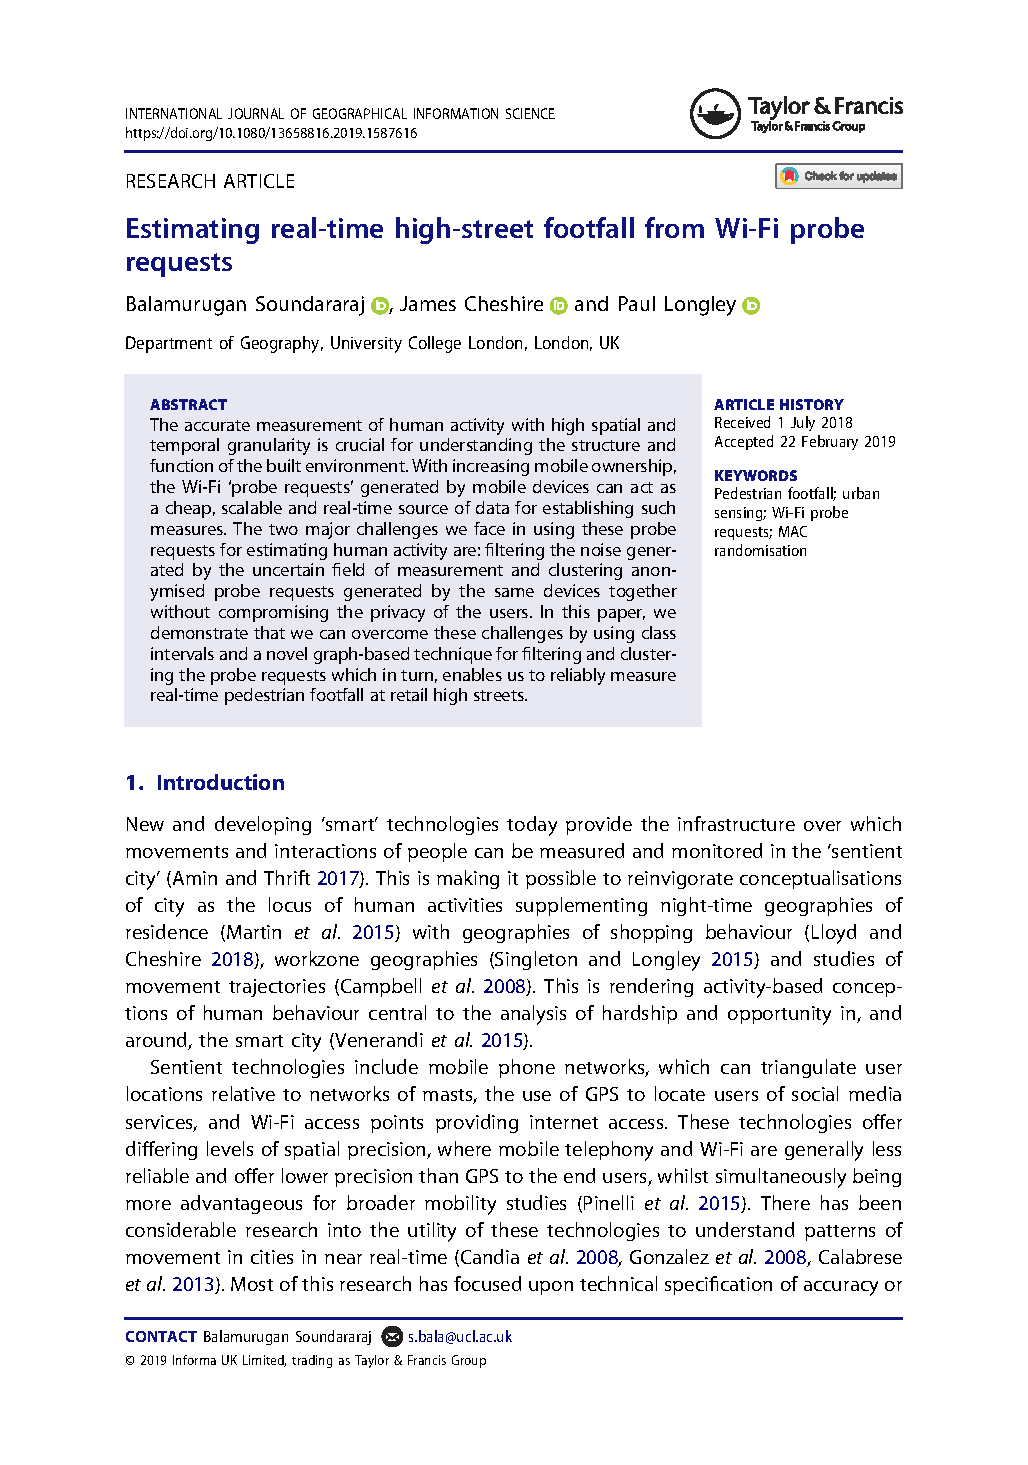
\includepdf[pages=1-15]{documents/ijgis-paper.pdf}
